%!TEX root =main.tex

\section{Lower bounding the expressive power}\label{sec:lowerb}

\floris{I think we need to show a lower bound for two classes. See later.
We may need to revise this section accordingly.}

We start this section by showing Theorem~\ref{thm:lowerb_general}.
More precisely, we show that for any given labeled graph
$(G,\pmb{\ell})$, there exist parameters $p$, $q$ and weight matrices $\mathbf{W}^{(t)}$, such that when $\mathbf{F}^{(0)}\equiv \hat{\pmb{\ell}}{}^{(t)}$, then for all $t\geq 0$, $\hat{\pmb{\ell}}{}^{(t)}\equiv \mathbf{F}^{(t)}$ where
$$
\mathbf{F}^{(t)}:=\sigma\left(\mathbf{L}(\mathbf{A}+p\mathbf{I})\mathbf{R}\mathbf{F}^{(t-1)}\mathbf{W}^{(t-1)} + q\mathbf{J}\right).$$ 

To show this, we follow the same strategy as in~\cite{grohewl}.
Crucial in establishing the lower bound are the following definitions (see also~\cite{grohewl}):
\begin{definition}[row independent modulo equality]\label{def:label2}\normalfont
A matrix $\mathbf{F}$ is \textit{row-independent modulo equality} if the unique row vectors in $\mathbf{F}$ are linearly independent. \qed
\end{definition}

\begin{definition}[a good matrix]\label{def:label3}\normalfont
A matrix $\mathbf{F}$ is \textit{good relative to an other matrix} $\mathbf{F}'$ if $\mathbf{F}\equiv \mathbf{F}'$ and $\mathbf{F}$ is row-independent modulo equality.\qed
\end{definition}

To show the lower bound we will inductively show that when $\mathbf{F}^{(t-1)}$ is good relative to $\hat{\pmb{\ell}}{}^{(t-1)}$, then. there exists a weight matrix $\mathbf{W}^{(t-1)}$, such that 
$\mathbf{F}^{(t)}$ is also good relative to $\hat{\pmb{\ell}}{}^{(t)}$. This clearly suffices to infer the lower bound. 

The induction hypothesis will be shown in a number of steps, by gradually adding the different components in the GNN architecture. We start by showing that multiplication with $\mathbf{R}$ preserves the goodness of the feature matrix.

%
% We first show, by induction on $t$, that when $\mathbf{F}^{(t)}$ is good relative to $\hat{\pmb{\ell}}^{(t)}$, then there exists a constant $p$ and constants $q^{(t)}$ and weight matrices
% $\mathbf{W}^{(t)}$, such that
% $$
% \mathbf{F}^{(t+1)}:=\sigma\Bigl(\mathbf{L}(\mathbf{A}+p\mathbf{I})\mathbf{R}\mathbf{F}^{(t)}\mathbf{W}^{(t)}+q^{(t)}\mathbf{B}\Bigr)
% $$
% is also good relative to $\hat{\pmb{\ell}}^{(t+1)}$. In a next step, we show that we can choose $q^{(t)}$ uniformly across all layers.


\begin{lemma}\label{lem:rightgood}
	For any $t\geq 0$,
	If $\mathbf{F}^{(t)}$ is good relative to $\hat{\pmb{\ell}}{}^{(t)}$, then $\mathbf{R}\mathbf{F}^{(t)}$ is also good relative to $\hat{\pmb{\ell}}{}^{(t)}$.
\end{lemma}
\begin{proof}
By assumption, we have that $\mathbf{F}^{(t)}_{v\bullet}=\mathbf{F}^{(t)}_{w\bullet}$ implies 
$\hat{\pmb{\ell}}{}^{(t)}_{v}=\hat{\pmb{\ell}}{}^{(t)}_w$. Furthermore, since $\hat{\pmb{\ell}}{}^{(t)}\sqsubseteq\hat{\pmb{\ell}}{}^{(0)}$,
$\mathbf{F}^{(t)}_{v\bullet}=\mathbf{F}^{(t)}_{w\bullet}$ implies  $\hat{\pmb{\ell}}{}^{(0)}_{v}=\hat{\pmb{\ell}}{}^{(0)}_w$. This in turn means that 
$\mathbf{R}_{vv}=\mathbf{R}_{ww}$. Hence, $\mathbf{F}^{(t)}_{v\bullet}=\mathbf{F}^{(t)}_{w\bullet}$  implies that 
$\mathbf{R}_{vv}\mathbf{F}^{(t)}_{v\bullet}=\mathbf{R}_{ww}\mathbf{F}^{(t)}_{w\bullet}$.
For the converse, suppose that $\mathbf{R}_{vv}\mathbf{F}^{(t)}_{v\bullet}=\mathbf{R}_{ww}\mathbf{F}^{(t)}_{w\bullet}$ holds.
Then, $\mathbf{F}^{(t)}_{v\bullet}=\mathbf{F}^{(t)}_{w\bullet}$ since otherwise we would have to
distinct rows $\mathbf{F}^{(t)}_{v\bullet}$ and $\mathbf{F}^{(t)}_{w\bullet}$ which are linearly dependent. This contradicts the assumption that $\mathbf{F}^{(t)}$ is row-independent modulo equality.
Hence, $\mathbf{R}\mathbf{F}^{(t)}\equiv\mathbf{F}^{(t)}\equiv\hat{\pmb{\ell}}{}^{(t)}$. Using the same reasoning as above, $\mathbf{R}\mathbf{F}^{(t)}$ is also row-independent modulo equality. Indeed, suppose that the unique rows in $\mathbf{R}\mathbf{F}^{(t)}$ are linearly dependent. Then, this implies that also the unique rows in $\mathbf{F}^{(t)}$ are linearly dependent, a contradiction. 
\end{proof}

We next consider multiplication with $\mathbf{A}+q\mathbf{I}$. 

\begin{lemma}\label{lem:findingp}
If $\mathbf{F}^{(t-1)}$ is good relative to $\hat{\pmb{\ell}}{}^{(t-1)}$, then there exists a  weight matrix $\mathbf{U}^{(t-1)}$ such that 
$\mathbf{G}^{(t)}:=(\mathbf{A}+p\mathbf{I})\mathbf{F}^{(t-1)}\mathbf{U}^{(t-1)}$ is equivalent to 
$\hat{\pmb{\ell}}{}^{(t)}$. Furthermore, this holds for any $p$ such that $0<p<1$.
\end{lemma}
\begin{proof}
By assumption, $\mathbf{F}^{(t-1)}$ is row-independent modulo equality.
Suppose that $\mathbf{F}^{(t-1)}$ is an $n\times f$-matrix, with $n$ the number of vertices in $(G,\pmb{\ell})$.
Let 
$\widetilde{\mathbf{F}}^{(t-1)}$ be the $u\times f$-matrix consisting of the unique rows in $\mathbf{F}^{(t-1)}$. Because the rows in $\widetilde{\mathbf{F}}^{(t-1)}$ are linearly independent,
there exists a $f\times u$-matrix $\mathbf{U}^{(t-1)}$ such that $\widetilde{\mathbf{F}}^{(t-1)}\mathbf{U}^{(t-1)}=\mathbf{I}_{u\times u}$. By induction $\mathbf{F}^{(t-1)}\equiv\hat{\pmb{\ell}}{}^{(t-1)}$. Let $\Sigma^{(t-1)}$ be the set of  labels assigned by $\hat{\pmb{\ell}}{}^{(t-1)}$ to vertices $v\in V$. 
For any $v\in V$ and $c\in\Sigma^{(t-1)}$, we denote by $\mathbf{F}^{(t-1)}_{v\bullet}\sim c$ that
$\hat{\pmb{\ell}}{}^{(t)}_v=c$.
Then for each $v\in V$ and $c\in \Sigma^{(t-1)}$ we have:
\begin{align*}
(\mathbf{A}\mathbf{F}^{(t-1)}\mathbf{M}^{(t-1)})_{vc}&=|\{u\in N_G(v)\mid \mathbf{F}^{(t-1)}_{u\bullet}\sim c\}|.
\intertext{Furthermore,} 
p\mathbf{I}(\mathbf{F}^{(t-1)}\mathbf{M}^{(t-1)})_{vc}&=p\delta_{vc},
\end{align*}
with $\delta_{vc}=1$ if $\mathbf{F}^{(t-1)}_{v\bullet}\sim c$ and $\delta_{vc}=0$ otherwise.

We next show that $\mathbf{G}^{(t)}:=(\mathbf{A}+p\mathbf{I})\mathbf{F}^{(t-1)}\mathbf{M}^{(t-1)}$ is equivalent to $\hat{\pmb{\ell}}{}^{(t)}$. Indeed, suppose that 
$\hat{\pmb{\ell}}{}^{(t)}_v=\hat{\pmb{\ell}}{}^{(t)}_w$. Then,
$\hat{\pmb{\ell}}{}^{(t-1)}_v=\hat{\pmb{\ell}}{}^{(t-1)}_w$ and for every $u\in N_G(v)$ and corresponding $u'\in N_G(w)$, $\hat{\pmb{\ell}}{}^{(t-1)}_u=\hat{\pmb{\ell}}{}^{(t-1)}_{u'}$. Since $\mathbf{F}^{(t-1)}\equiv\hat{\pmb{\ell}}{}^{(t-1)}$ this implies for any $c\in \Sigma^{(t-1)}$,
 $\delta_{vc}=\delta_{wc}$ and 
$|\{u\in N_G(v)\mid \mathbf{F}^{(t-1)}_{u\bullet}\sim c\}|=
|\{u\in N_G(w)\mid \mathbf{F}^{(t-1)}_{u\bullet}\sim c\}|$. In other words,
$\mathbf{G}^{(t)}_{v\bullet}=\mathbf{G}^{(t)}_{w\bullet}$. Conversely,
suppose that $\mathbf{G}^{(t)}_{v\bullet}=\mathbf{G}^{(t)}_{w\bullet}$. Then, for every $c\in \Sigma^{(t-1)}$,
$|\{u\in N_G(v)\mid \mathbf{F}^{(t-1)}_{u\bullet}\sim c\}|+p\delta_{vc}=
|\{u\in N_G(w)\mid \mathbf{F}^{(t-1)}_{u\bullet}\sim c\}|+p\delta_{wc}$. We next distinguish between a number of cases. Suppose first that $\delta_{vc}=\delta_{wc}$. Then, we must have that $|\{u\in N_G(v)\mid \mathbf{F}^{(t-1)}_{u\bullet}\sim c\}|=
|\{u\in N_G(w)\mid \mathbf{F}^{(t-1)}_{u\bullet}\sim c\}|$. Since $\mathbf{F}^{(t-1)}\equiv\hat{\pmb{\ell}}^{(t-1)}$ this implies that $\hat{\pmb{\ell}}{}^{(t-1)}_v=\hat{\pmb{\ell}}{}^{(t-1)}_w$ and for every $u\in N_G(v)$ and corresponding $u'\in N_G(w)$, $\hat{\pmb{\ell}}{}^{(t-1)}_u=\hat{\pmb{\ell}}{}^{(t-1)}_{u'}$. In other words, 
$\hat{\pmb{\ell}}{}^{(t)}_v=\hat{\pmb{\ell}}{}^{(t)}_w$. By contrast, if $\delta_{vc}\neq \delta_{wc}$ then either $|\{u\in N_G(v)\mid \mathbf{F}^{(t-1)}_{u\bullet}\sim c\}|=
|\{u\in N_G(w)\mid \mathbf{F}^{(t-1)}_{u\bullet}\sim c\}|+p$ or
$|\{u\in N_G(v)\mid \mathbf{F}^{(t-1)}_{u\bullet}\sim c\}|+p=
|\{u\in N_G(w)\mid \mathbf{F}^{(t-1)}_{u\bullet}\sim c\}|$. This, however, is impossible for any $p$ such that $0<p<1$ because  $|\{u\in N_G(w)\mid \mathbf{F}^{(t-1)}_{u\bullet}\sim c\}|$ and $|\{u\in N_G(w)\mid \mathbf{F}^{(t-1)}_{u\bullet}\sim c\}|$ are integers.
\end{proof}


We remark that the previous lemma only guarantees that $\mathbf{H}^{(t)}$ is equivalent to $\hat{\pmb{\ell}}{}^{(t)}$. We show later how row-independence modulo equality is ensured.
Furthermore, the lemma is stated in terms of $\mathbf{F}^{(t)}$ instead of $\mathbf{R}\mathbf{F}^{(t)}$.
From Lemma~\ref{lem:rightgood} we know, however, that $\mathbf{F}^{(t)}\equiv\mathbf{R}\mathbf{F}^{(t)}$
so we can apply Lemma~\ref{lem:findingp} to $\mathbf{R}\mathbf{F}^{(t)}$ as well.

We next consider multiplication with $\mathbf{L}$. In the following, we let $\mathbf{G}^{(t)}:=(\mathbf{A}+p\mathbf{I})\mathbf{R}\mathbf{F}^{(t-1)}\mathbf{U}^{(t-1)}$.

% \todo{The lemma below is new. It allows to use a simplified bias matrix. Our previous argument required the bias matrix to be $\mathbf{L}\mathbf{J}$. We now only have $\mathbf{J}$. This lemma needs to be checked carefully ;-)}
\begin{lemma}\label{lemma:findp}
There exists a constant $m_p$, only dependent on $\mathbf{L}$ and the number of vertices $V$ in $G$, such that for all $p$ for which $m_p<p<1$, $\mathbf{L}\mathbf{G}^{(t)}$ is equivalent to $\hat{\pmb{\ell}}{}^{(t)}$.
\end{lemma}
\begin{proof}
	We know from Lemma~\ref{lem:findingp} that
 $\mathbf{G}^{(t)}\equiv\hat{\pmb{\ell}}{}^{(t)}$ for all $p$, $0<p<1$.
	Suppose that $\hat{\pmb{\ell}}{}^{(t)}_v=\hat{\pmb{\ell}}{}^{(t)}_w$, or equivalently, that	$\mathbf{G}^{(t)}_{v\bullet}=\mathbf{G}^{(t)}_{w\bullet}$. This implies that
	  $\hat{\pmb{\ell}}{}^{(0)}_v=\hat{\pmb{\ell}}{}^{(0)}_w$. In particular, we must have that $\mathbf{L}_{vv}=\mathbf{L}_{ww}$. This in turn implies
$\mathbf{L}_{vv}\mathbf{G}^{(t)}_{v\bullet}=\mathbf{L}_{ww}\mathbf{G}^{(t)}_{w\bullet}$.

We next describe a procedure of how to obtain $m_p$. Later on, we define $m_p$ directly
from $\mathbf{L}$ and $n$.

Initially, $m_p=0$. Then, we update $m_p$ as long as
$\mathbf{L}\mathbf{G}^{(t)}\not\equiv\hat{\pmb{\ell}}{}^{(t)}$. We have just seen that
$\hat{\pmb{\ell}}{}^{(t)}\sqsubseteq \mathbf{L}\mathbf{G}^{(t)}$ for all $p$, $0<p<1$.
Hence, we update $m_p$ as long as $\mathbf{L}\mathbf{G}^{(t)}\not\sqsubseteq\hat{\pmb{\ell}}{}^{(t)}$.
The latter implies that
there exists two vertices $v,w\in V$ such that
\begin{equation}
\mathbf{L}_{vv}\mathbf{G}^{(t)}_{v\bullet}=\mathbf{L}_{ww}\mathbf{G}^{(t)}_{w\bullet},\label{eq:contra}
\end{equation}
but $\hat{\pmb{\ell}}{}^{(t)}_v\neq \hat{\pmb{\ell}}{}^{(t)}_w$, or equivalently, $\mathbf{G}^{(t)}_{v\bullet}\neq \mathbf{G}^{(t)}_{w\bullet}$.
Clearly, in this case $\mathbf{L}_{vv}\neq\mathbf{L}_{ww}$. Hence, the equality~(\ref{eq:contra}) implies that for every $c\in\Sigma^{(t-1)}$, either
(i)~$\mathbf{G}^{(t)}_{vc}=0=\mathbf{G}^{(t)}_{wc}$; or (ii)~ $0\neq \mathbf{G}^{(t)}_{vc}\neq \mathbf{G}^{(t)}_{wc}\neq 0$. Here, $\Sigma^{(t-1)}$ is the set of labels as used in the proof of  Lemma~\ref{lem:findingp}. Furthermore, for all $c\in\Sigma^{(t-1)}$ for which (ii) holds, 
\begin{equation}
\frac{\mathbf{G}^{(t)}_{vc}}{\mathbf{G}^{(t)}_{wc}}=\frac{\mathbf{L}_{ww}}{\mathbf{L}_{vv}}\neq 1.\label{eq:ratio}
\end{equation}
Let $\alpha:=\frac{\mathbf{L}_{ww}}{\mathbf{L}_{vv}}$.
We also observe that, since $p$ occurs in precisely one entry in $\mathbf{G}^{(t)}_{v\bullet}$ and $\mathbf{G}^{(t)}_{w\bullet}$, there is at least one $c\in\Sigma^{(t-1)}$ for which (ii) holds. Furthermore, the proof of  Lemma~\ref{lem:findingp} tells precisely how the elements $\mathbf{G}^{(t)}_{vc}$ and $\mathbf{G}^{(t)}_{wc}$ look like. That is, these entries are of the form 
$i$ or $i+p$ for $i\in[1,n]$ with $n=|V|$. If we consider equation~(\ref{eq:ratio}) for
the entries containing $p$ we are in one of the following three cases:
$$
\text{(a) } \frac{i+p}{j}=\alpha
\text{; (b) } \frac{i}{j+p}=\alpha
\text{; or (c) } \frac{i+p}{j+p}=\alpha
$$
for some $i,j\in[1,n]$. Hence, in case (a)~$p=\alpha j- i$, in case (b)~$p=\frac{i-\alpha j}{\alpha}$, and in case (c)~$p=\frac{\alpha(j-i)}{1-\alpha}$. It now suffices to update
$m_p=\max\{m_p,\alpha j- i,\frac{i-\alpha j}{\alpha},\frac{\alpha(j-i)}{1-\alpha}\}$ and
hence for any $p>m_p$, equation~(\ref{eq:ratio}) is not satisfied anymore for $v$ and $w$.
We proceed in this way, as long is there exists a pair of vertices  $v,w\in V$ for which equation~\ref{eq:contra} holds  but $\hat{\pmb{\ell}}{}^{(t)}_v\neq \hat{\pmb{\ell}}{}^{(t)}_w$. Note that $m_p$ has been updated for a particular pair of vertices, that pair will not need to considered anymore. The final $m_p$ is the value when
for all vertices $v,w\in V$, equation~\ref{eq:contra} implies $\hat{\pmb{\ell}}{}^{(t)}_v= \hat{\pmb{\ell}}{}^{(t)}_w$. In other words, when $\mathbf{L}\mathbf{G}^{(t)}\sqsubseteq\hat{\pmb{\ell}}{}^{(t)}$ holds.

It should be clear now that we can define $m_p$ more roughly, as follows.
First, define $L':=\{\frac{\mathbf{L}_{vv}}{\mathbf{L}_{ww}}\mid \mathbf{L}_{vv}\neq\mathbf{L}_{ww}, v,w\in V\}$. Then, consider
\begin{align*}
P_1&:=\left\{ \alpha j -i \mid 0\leq \alpha i -j < 1, i,j\in[1,n],\alpha\in L'\right\}\\
P_2&:=\left\{ \frac{i -\alpha j}{\alpha} \mid 0\leq \frac{i -\alpha j}{\alpha} < 1, i,j\in[1,n],\alpha\in L'\right\}\\
P_3&:=\left\{ \frac{\alpha(j-i)}{1-\alpha} \mid 0\leq \frac{\alpha(j-i)}{1-\alpha} < 1, i,j\in[1,n],\alpha\in L'\right\}
\end{align*}
and let $m_p=\max\{P_1\cup P_2\cup P_3\cup\{0\}\}$. In other words, we just consider all possible $p$ values as determined before that could lead to 
$\mathbf{L}\mathbf{G}^{(t)}\not\sqsubseteq\hat{\pmb{\ell}}{}^{(t)}$ and eliminate these possibility by choosing $p$ large enough, as explained earlier.
%
% We will sho
% consider the set $L':=\{\frac{\mathbf{L}_{vv}}{\mathbf{L}_{ww}}\mid \mathbf{L}_{vv}\neq\mathbf{L}_{ww}, v,w\in V\}$. We remark this, by assumption $L_{vv}\neq 0$ for any $v\in V$ so we do not have zero denominators. We define $m_p$ as follows.
% Initially, we set $m_p:0$. Then,
% suppose that
% $\mathbf{L}_{vv}\mathbf{G}^{(t)}_{v\bullet}=\mathbf{L}_{ww}\mathbf{G}^{(t)}_{w\bullet}$ for some
% vertices $v,w\in V$. We will show how to change $m_p$ such for all $p$ satisfying
% $m_p<p<1$, $\mathbf{L}_{vv}\mathbf{G}^{(t)}_{v\bullet}\neq \mathbf{L}_{ww}\mathbf{G}^{(t)}_{w\bullet}$.
% (Recall from the proof of  Lemma~\ref{lem:findingp} that every $\mathbf{G}^{(t)}_{v\bullet}$
% has at least one entry containing $p$.)
%
%
%
%
% We next consider $M'=\{\frac{\mathbf{G}^{(t)}_{wc}}{\mathbf{G}^{(t)}_{vc}}\mid \mathbf{G}^{(t)}_{vc}\neq \mathbf{G}^{(t)}_{wc},\mathbf{G}^{(t)}_{vc}\neq 0, v,w\in V,c\in\Sigma^{(t-1)}\}$, where $\Sigma^{(t-1)}$ is the set of labels as used in the proof of  Lemma~\ref{lem:findingp}. From that proof we also know precisely how the ratio's in $M'$ look like. That is, every such a ratio is of the form
% $\frac{i+p}{j}$, $\frac{i}{j+p}$ or $\frac{i+p}{j+p}$ for $i,j\in[0,|V|]$.
%
%  Let
% $G$ be the collection of all these fractions and choose $p$ such that $G\cap L'=\emptyset$
% (almost any $p$ will do.). Suppose now that $\hat{\pmb{\ell}}^{(t)}_v\neq \hat{\pmb{\ell}}^{(t)}_w$
% and thus $\mathbf{G}^{(t)}_{v\bullet}\neq \mathbf{G}^{(t)}_{w\bullet}$. Suppose, for the sake of
% contradiction that $\mathbf{L}_{vv}\mathbf{G}^{(t)}_{v\bullet}=\mathbf{L}_{ww}\mathbf{G}^{(t)}_{w\bullet}$. This implies
% that the non-zero entries in $\mathbf{G}^{(t)}_{v\bullet}$ correspond to non-zero (but possibly different)
% entries in $\mathbf{G}^{(t)}_{w\bullet}$. We are guaranteed at least one non-zero entry in $\mathbf{G}^{(t)}_{v\bullet}$ which contains $p$. Assume that this entry is of the form $i+p$. Then,
% the corresponding non-zero entry in $\mathbf{G}^{(t)}_{w\bullet}$ is of the form $j$ or $j+p$. We also know that  $\mathbf{G}^{(t)}_{v\bullet}\neq \mathbf{G}^{(t)}_{w\bullet}$ and $\mathbf{L}_{vv}\mathbf{G}^{(t)}_{v\bullet}=\mathbf{L}_{ww}\mathbf{G}^{(t)}_{w\bullet}$ implies that
% $\mathbf{L}_{vv}\neq\mathbf{L}_{ww}$. Hence, the assumption implies that
% $\frac{\mathbf{L}_{vv}}{\mathbf{L}_{ww}}=\frac{j}{i+p}$ or $\frac{\mathbf{L}_{vv}}{\mathbf{L}_{ww}}=\frac{j+p}{i+p}$. In other words, $G\cap L'\neq\emptyset$, a contradiction.
\end{proof}

At this point, we know that when $\mathbf{F}^{(t-1)}$ is good relative to $\hat{\pmb{\ell}}{}^{(t-1)}$ then there exists a $\mathbf{M}^{(t-1)}$ such that $\mathbf{H}^{(t)}:=\mathbf{L}(\mathbf{A}+p\mathbf{I})\mathbf{R}\mathbf{F}^{(t-1)}\mathbf{M}^{(t-1)}$
is equivalent to $\hat{\pmb{\ell}}{}^{(t)}$, and this for any $p$ such that $m_p<p<1$.
We now come to the point that will ensure that there exists a $q$ and $\mathbf{N}^{(t-1)}$ such that
$$
\mathbf{F}^{(t)}:=\sigma(\mathbf{L}(\mathbf{A}+p\mathbf{I})\mathbf{R}\mathbf{F}^{(t-1)}\underbrace{\mathbf{M}^{(t-1)}\mathbf{N}^{(t-1)}}_{\mathbf{W}^{(t-1)}}+q\mathbf{J})$$
 is good relative to $\hat{\pmb{\ell}}{}^{(t)}$, where $\sigma$ is either the sign or the ReLU activation function. We here follow closely the approach taken in~\cite{grohewl}.
Lemma 9 in~\cite{grohewl} states:

 \begin{lemma}[Lemma 9 in~\cite{grohewl}]\label{lem:signlemma9}
  Let
  $\mathbf{B}\in \Nb^{u\times f}$ be a matrix in which all
  rows are pairwise disjoint.
%  \footnote{I believe that this can be
%  guaranteed in 1-WL}).\todo{G: with our extended features we actually guarantee this for free by adding the 1 column; also, t as dimension is a bad choice\ldots}
  Then there exists a matrix $\mathbf{N}$ 
  such that $\text{\normalfont sign}(\mathbf{BN}-\mathbf{J})$ is
  non-singular.
\end{lemma}
Although~\cite{grohewl} also consider the ReLU activation function, they simulate each application of the ReLu function by two applications of the sign function. As a consequence,
the overall number of layers doubled. A more direct approach can be applied, however. More
precisely, we show the following:
 \begin{lemma}\label{lem:relulemma9}
  Let
  $\mathbf{B}\in \Nb^{u\times f}$ be a matrix in which all
  rows are pairwise disjoint and such that no row consists entirely
  out of zeroes.
%  \footnote{I believe that this can be
%  guaranteed in 1-WL}).\todo{G: with our extended features we actually guarantee this for free by adding the 1 column; also, t as dimension is a bad choice\ldots}
  Then there exists a matrix $\mathbf{N}$ and a constant $q$
  such that $\text{\normalfont ReLU}(\mathbf{BN}-q\mathbf{J})$ is
  non-singular. In fact, if we denote by $M$ the maximal entry in $\mathbf{B}$,
  any $q$ such that  $\frac{M^f-1}{M^f} < q < 1$ will do.
\end{lemma}
\begin{proof}
Let $M$ be the maximal entry in $\mathbf{B}$ and consider the column vector $\mathbf{z}=(1,M,M^2,\ldots,M^{f-1})^{\textsc{t}}$.
Then each entry in $\mathbf{b}=\mathbf{B}\mathbf{z}$ is positive and they are all pairwise distinct. 
Let $\mathbf{P}$ be a permutation matrix in $\Rb^{u\times u}$ such that $\mathbf{b}'=\mathbf{P}\mathbf{b}$ is such that  $\mathbf{b}'=(b_1',b_2',\ldots,b_u')^{\textsc{	t}}\in\Rb^{u\times 1}$ with $ b_1'> b_2'>\cdots > b_u'>0$. 
Consider the $\mathbf{x}=\left(\frac{1}{b_1'},\ldots,\frac{1}{b_u'}\right)\in \Rb^{1\times u}$. Then, for $\mathbf{C}=\mathbf{b}'\mathbf{x}$
$$
\mathbf{C}_{ij}=\frac{b_i'}{b_j'}  \text{ and } \mathbf{C}_{ij}=\begin{cases}  1 & \text{if $i=j$}\\
>1 & \text{if $i<j$}\\
< 1 & \text{if $i>j$}.
\end{cases}
$$
Let $q$ be the greatest value  in $\mathbf{C}$ smaller than $1$.
% G: I think the m instantiated here is not correct
%, i.e., $m=\frac{b_s}{b_1}$.
Consider $\mathbf{E}=\mathbf{C}- q\mathbf{J}$.
Then,
$$
\mathbf{E}_{ij}=\frac{b_i'}{b_j'}- q \text{ and } \mathbf{E}_{ij}=\begin{cases}  1-m & \text{if $i=j$} \\
> 0 & \text{if $i<j$}\\
\leq 0  & \text{if $i>j$}.
\end{cases}
$$
As a consequence,
$$
\text{ReLU}(\mathbf{E})_{ij}=\begin{cases}  1-q & \text{if $i=j$}\\
>0 & \text{if $i<j$}\\
0  & \text{if $i>j$}.
\end{cases}
$$
This is an upper triangular matrix with (nonzero) value $1-q$ on its diagonal. It is therefore non-singular. 
We observe that $\mathbf{Q}\text{ReLU}(\mathbf{E})=\text{ReLU}(\mathbf{Q}\mathbf{E})$ for any row permutation $\mathbf{Q}$. Furthermore, non-singularity is preserved under row permutations and $\mathbf{Q}\mathbf{J}=\mathbf{J}$. Hence, if we define $\mathbf{N}=\mathbf{z}\mathbf{x}$ and use the permutation matrix $\mathbf{P}$:
\begin{align*}
\mathbf{P}\text{ReLU}(\mathbf{B}\mathbf{N}-q\mathbf{J})&=
\text{ReLU}(\mathbf{P}\mathbf{B}\mathbf{z}\mathbf{x}-q\mathbf{P}\mathbf{J})=\text{ReLU}(\mathbf{E}-q\mathbf{J}),
\end{align*}
we have that $\text{ReLU}(\mathbf{B}\mathbf{N}-q\mathbf{J})$ is non-singular, as desired.
%So, the lemma is satisfied by taking $m$ as above and
%%$m=b_s/b_1$ and % G: this still looks wrong
%$\mathbf{X}=\mathbf{z}\mathbf{x}$.
To validate second claim in the statement of the lemma, it suffices to observe that every
in $\mathbf{b'}$ is bounded by $M^f$ and hence every 
$\frac{b_i'}{b_j'}$ in $\mathbf{C}$ such that $\frac{b_i'}{b_j'}<1$ is bounded by
$\frac{M^f-1}{M^f}$. Choosing $q$ larger than this number clearly
ensures the correctness of the above construction.
\end{proof}

We are now almost at the end of the lower bound proof. Indeed,
consider the matrix $\widetilde{\mathbf{H}}{}^{(t)}$ consisting of the unique rows
of $\mathbf{H}^{(t)}:=\mathbf{L}(\mathbf{A}+p\mathbf{I})\mathbf{R}\mathbf{F}^{(t-1)}\mathbf{M}^{(t-1)}$. Suppose that $\widetilde{\mathbf{H}}{}^{(t)}$ is of dimension $u\times f$.
Then, when $\sigma$ is the sign function, Lemma~\ref{lem:signlemma9} implies 
the existence of an $f\times u$-matrix $\mathbf{N}^{(t)}$ such that
$\sigma(\widetilde{\mathbf{H}}{}^{(t)}\mathbf{N}^{(t)}-\mathbf{J})$ is non-singular
and thus is row-independent. As a consequence, 
$\mathbf{F}^{(t)}:=\sigma(\mathbf{H}{}^{(t)}\mathbf{N}^{(t)}-\mathbf{J})$ is 
row-independent modulo equality. Since  $\mathbf{H}{}^{(t)}\equiv\hat{\pmb{\ell}}{}^{(t)}$
we have that there is a bijection between $\widetilde{\mathbf{H}}{}^{(t)}$ and the labels
used by $\hat{\pmb{\ell}}{}^{(t)}$. There are $u$ such labels and these again bijectively
map on $\sigma(\widetilde{\mathbf{H}}{}^{(t)}\mathbf{N}^{(t)}-\mathbf{J})$.
It now easily follows that
$\mathbf{F}^{(t)}\equiv\hat{\pmb{\ell}}{}^{(t)}$ as well.

When the activation function is ReLU, we will apply Lemma~\ref{lem:relulemma9} in precisely the same way. We first remark that $\widetilde{\mathbf{H}}{}^{(t)})$ does not contain rows consisting of zeroes only. Indeed, there is at least one entry that has the $p$ parameter.
\marginpar{We do not self-loop assumption, it seems.}
We note, however, that this lemma provides a different lower bound for $q$ in each layer. It suffices to observe $(\widetilde{\mathbf{H}}{}^{(t)})_{v,c}$ is either of the form $\mathbf{L}_{vv}(i+p)$ or $\mathbf{L}_{vv}(i)$ for some $i\in [1,n]$. This holds for every $t\geq 0$. Hence, we know that for all $t\geq 0$, the elements in 
$\widetilde{\mathbf{H}}{}^{(t)}$ are upper bounded by $\ell(n+1)$ where $\ell=\max\{\mathbf{L}_{vv}\mid v\in V\}$. As a consequence, we can take 
$\frac{(\ell(n+1))^f-1}{(\ell(n+1))^f}$ as the lower bound for $q$, independent of layer under consideration.

This concludes the proof of  Theorem~\ref{thm:lowerb_general}.
%
% are of the $\ell(i+p)$ or $\ell i$ where
% It now suffices to apply this Lemmas for the matrix $\mathbf{B}$ consisting of the unique rows of $\mathbf{H}^{(t)}:=\mathbf{L}(\mathbf{A}+p\mathbf{I})\mathbf{R}\mathbf{F}^{(t-1)}\mathbf{M}^{(t-1)}$. Then, we define  $\mathbf{N}^{(t-1)}:=\mathbf{X}$ and take $q> \frac{M^q-1}{M^q}$
% as given by the lemma.
%
% The Lemma then guarantees that $\mathbf{F}^{(t+1)}$ is row-independent modulo equality. Furthermore,
% we have that $\sigma(\mathbf{H}^{(t)}\mathbf{N}^{(t)}+q^{(t)}\mathbf{J})\equiv \mathbf{H}^{(t)}$ and
% thus $\mathbf{F}^{(t+1)}\equiv\hat{\pmb{\ell}}^{(t+1)}$, as desired.
%
% As anticipated, we finally argue that the parameters $q^{(t)}$ can be chosen uniformly across all layers.
% If we inspect the proof of Lemma~\ref{lem:relulemma9} then the constant $m$ needs to be chosen such that
% it is (i)~smaller than $1$ and (ii)~larger than any ratio $\mathbf{C}_{vw}=\mathbf{b}_{v}/\mathbf{w}$, where $\mathbf{b}$ is obtained based on $\mathbf{B}$ and $M$, an upper bound on the largest number in $\mathbf{B}$.
%
% As mentioned earlier, we apply  Lemma~\ref{lem:relulemma9} for $\mathbf{B}=\mathbf{H}^{(t)}$.
% For each $t\geq 0$, we know that
% $$\mathbf{B}_{vc}=\mathbf{L}_{vv}|\{u\in N_G(v)\mid \mathbf{F}^{(t)}_{v\bullet}\sim c\}|+\delta_{vc}p
% \leq \ell(|V|+1),
% $$
% with $\ell:=\max\{\mathbf{L}_{vv}\mid v\in V\}$. Let $M=\ell(|V|+1)$. Following the proof of Lemma~\ref{lem:relulemma9} we thus have that every element in $\mathbf{H}^{(t)}\mathbf{b}$ is
% of the form $\sum_{i=1}^{n-1}\alpha_i M^i$ and is thus smaller than $M^n$. This implies that the
% largest ratio of elements in $\mathbf{H}^{(t)}\mathbf{b}$, smaller than $1$, is upper bounded by
% $\frac{M^n-1}{M^n}$. In other words,
% \begin{lemma}
% If we choose $q> \frac{(\ell(|V|+1))^n-1}{(\ell(|V|+1))^n}$, then for any $t\geq 0$, there exists a matrix $\mathbf{X}^{(t)}$ such that $\text{ReLU}(\tilde{\mathbf{H}^{(t)}}\mathbf{X}^{(t)}-q\mathbf{J})$
% is non-singular, where $\tilde{\mathbf{H}^{(t)}}$ denotes the matrix consisting of unique rows from
% $\mathbf{H}^{(t)}$ and $\ell=\max\{\mathbf{L}_{vv}\mid v\in V\}$.
% \end{lemma}
%

\floris{I don't know whether the following is of interest. We have a stronger lower bound than in~\cite{grohewl}. More specifically, we assume only one weight matrix (instead of two) and furthermore, can assume this weight matrix to be a rank one matrix. This implies that it is the product of two vectors, reducing $n^2$ parameters to $2n$! It may be interesting to see how this simple architecture behaves in practice....}

\begin{theorem}
GNN architectures of the $\mathbf{F}^{(t)}:=\sigma\bigl((\mathbf{A}+p\mathbf{I})\mathbf{F}^{(t-1)}\mathbf{W}^{(t-1)} +q\mathbf{J}\bigr)$ with $\mathbf{W}$ a rank-one matrix, is WL-strong, for any $0<p<1$ and $m_q<q<1$ for some $m_q$.
\end{theorem}
\begin{proof}
We assume that $\mathbf{F}^{(0)}\equiv\pmb{\ell}$ and that  $\mathbf{F}^{(0)}$ is row-independent modulo equality. We define for $t>0$:
	\begin{align*}
	\mathbf{G}^{(t)}&:=(\mathbf{A}+p\mathbf{I})\mathbf{F}^{(t-1)}\\
	\mathbf{F}^{(t)}&:=\sigma(\mathbf{G}^{(t)}\mathbf{W}^{(t-1)}+q\mathbf{J}).
	\end{align*}
We assume next that $\mathbf{F}^{(t-1)}$ is good for $\pmb{\ell}{}^{(t-1)}$. We first show that
$\mathbf{G}^{(t)}\equiv\pmb{\ell}^{(t)}$, and then apply
	Lemmas~\ref{lem:signlemma9} and
	~\ref{lem:relulemma9} to find $\mathbf{W}^{(t-1)}$ and $q$ such that $\mathbf{F}^{(t)}$ is good for  $\pmb{\ell}{}^{(t)}$. We observe that these lemmas create a rank one matrix $\mathbf{W}^{(t-1)}$.


We observe that the upper bound proof of Theorem~\ref{thm:generalbound}  implies that  $\pmb{\ell}{}^{(t)}\sqsubseteq \mathbf{G}^{(t)}$. It thus suffices to show that $ \mathbf{G}^{(t)}\sqsubseteq \pmb{\ell}{}^{(t)}$.

Suppose, for the sake of contradiction, that there exists two vertices $v,w\in V$ such that 
	\begin{equation}
	\pmb{\ell}{}^{(t)}_v\neq\pmb{\ell}{}^{(t)}_w \text{ and }
	\mathbf{G}^{(t)}_{v\bullet}=\mathbf{G}^{(t)}_{w\bullet}. \label{eq:contra}
	\end{equation} 
We show that this is impossible for $p$ such that $0<p<1$. We distinguish between the following two cases. If $\pmb{\ell}{}^{(t)}_v\neq\pmb{\ell}{}^{(t)}_w$ then either
(i)~$\pmb{\ell}{}^{(t-1)}_v\neq\pmb{\ell}{}^{(t-1)}_w$; or 
(ii)~$\pmb{\ell}{}^{(t-1)}_v=\pmb{\ell}{}^{(t-1)}_w$ and
	$$
	\ldbl \pmb{\ell}{}^{(t-1)}_{u} \st u \in N_G(v) \rdbl\neq
	\ldbl \pmb{\ell}{}^{(t-1)}_{u} \st u \in N_G(w) \rdbl.
	$$
By assumption $\mathbf{F}^{(t-1)}$ is good for $\pmb{\ell}{}^{(t-1)}$.
In particular, if we consider the unique row vectors in  $\mathbf{F}^{(t-1)}$, then these are linearly independent. Let us denote the unique row vectors in $\mathbf{F}^{(t-1)}$ by $\mathbf{F}_1,\ldots,\mathbf{F}_s$ for some $s$.


Suppose that we are in case (i). Then,  $\pmb{\ell}{}^{(t-1)}_v\neq\pmb{\ell}{}^{(t-1)}_w$ implies that
	$\mathbf{F}^{(t-1)}_{v\bullet}\neq \mathbf{F}^{(t-1)}_{w\bullet}$. We can assume, wlog, that $\mathbf{F}^{(t-1)}_{v\bullet}=\mathbf{F_1}$ and
	$\mathbf{F}^{(t-1)}_{w\bullet}=\mathbf{F_2}$. It should be clear from the definition of $\mathbf{G}^{(t)}$ that every of its rows is a linear combination of 
	the unique row vectors $\mathbf{F}_1,\ldots,\mathbf{F}_s$. More specifically:
	\begin{align*}
	\mathbf{G}^{(t)}_{v\bullet}&:=(\alpha_1+p)\mathbf{F}_1+ \alpha_2\mathbf{F}_2+ \sum_{i=3}^s \alpha_i\mathbf{F}_i\\
	%\intertext{and similarly,} 
	\mathbf{G}^{(t)}_{w\bullet}&=\beta_1\mathbf{F}_1+ (\beta_2+p)\mathbf{F}_2+ \sum_{i=3}^s \beta_i\mathbf{F}_i,
	\end{align*}
	for some non-negative natural numbers $\alpha_i$ and $\beta_i$, for $i\in[1,s]$.
We recall, however, that the vertices $v$ and $w$ are such that $\mathbf{G}^{(t)}_{v\bullet}=\mathbf{G}^{(t)}_{w\bullet}$. This in turn implies that
	$$
	(\alpha_1+p-\beta_1)\mathbf{F}_1 + (\alpha_2-\beta_2-p)\mathbf{F}_2 +\sum_{i=3}^s (\alpha_i-\beta_i)\mathbf{F}_s=0.
	$$
	So, unless all these coefficients are zero, we have that $\mathbf{F}_1,\ldots,\mathbf{F}_s$
	are not linearly independent. It is now clear that $\alpha_1+p=\beta_1$ and
	$\alpha_2=\beta_2+p$ cannot hold for any $p$, $0<p<1$. Indeed, $\alpha_i-\beta_j$
	is always an integer number. Hence, case (i) cannot occur.
	

Suppose next that we are in case (ii). Recall that for case (ii), we have $\pmb{\ell}{}^{(t-1)}_v=\pmb{\ell}{}^{(t-1)}_w$.
	Using the same notation as above, we may assume that $\mathbf{F}^{(t-1)}_{v\bullet}=\mathbf{F_1}=\mathbf{F}^{(t-1)}_{w\bullet}$. In case (ii), however, we have that
	$
	\ldbl \pmb{\ell}{}^{(t-1)}_{u} \st u \in N_G(v) \rdbl\neq
	\ldbl \pmb{\ell}{}^{(t-1)}_{u} \st u \in N_G(w) \rdbl
	$.
	That is, there must exist a label assigned by $\pmb{\ell}{}^{(t-1)}$ that does not occurs the same number of times in the neighborhoods of $v$ and $w$, respectively. Recall that $\mathbf{F}^{(t-1)}\equiv \pmb{\ell}{}^{(t-1)}$. We assume that $\mathbf{F}_2$ corresponds to the label witnessing the difference in the neighborhood labels. (As a special case, this label may also correspond to $\mathbf{F}_1$ but the same argument as below applies.)

We develop $\mathbf{G}^{(t)}_{v\bullet}$ and $\mathbf{G}^{(t)}_{w\bullet}$ again as linear combinations of $\mathbf{F}_1,\ldots,\mathbf{F}_s$. That is,
	\begin{align*}
	\mathbf{G}^{(t)}_{v\bullet}&:=(\alpha_1+p)\mathbf{F}_1+ \alpha_2\mathbf{F}_2+ \sum_{i=3}^s \alpha_i\mathbf{F}_i\\
	%\intertext{and similarly,} 
	\mathbf{G}^{(t)}_{w\bullet}&=(\beta_1+p)\mathbf{F}_1+ \beta_2\mathbf{F}_2+ \sum_{i=3}^s \beta_i\mathbf{F}_i.
	\end{align*}
	Our assumption (also in case (ii)) is still that $\mathbf{G}^{(t)}_{v\bullet}=\mathbf{G}^{(t)}_{w\bullet}$. Using the same argument as before, based on linear independence of $\mathbf{F}_1,\ldots,\mathbf{F}_s$, we must have that 
	$\alpha_i=\beta_i$ for all $i\in [1,s]$.
This cannot be true, however. Indeed,
 $\alpha_2$ and $\beta_2$, corresponding to $\mathbf{F}_2$, correspond to the number of time the label corresponding to $\mathbf{F}_2$ occurs in $N_G(u)$ and $N_G(w)$, respectively. By assumption, these numbers are different. So again, case (ii) cannot occur either. Hence, $\mathbf{G}^{(t)}\sqsubseteq \pmb{\ell}^{(t)}$, as desired.
\end{proof}


\floris{The lower bound so far do not cover the two GCN cases. Question: 
Can the lower bound be established also for 
$$
\mathbf{F}^{(t)}:=\sigma((\mathbf{L}\mathbf{A}\mathbf{R}+p\mathbf{I})\mathbf{F}^{(t-1)}\mathbf{W}^{(t-1)}+q\mathbf{J})??
$$. I believe what is written below works. In fact, I think we can use this approach also for the other lower bound. It may simplify matter. {\bf FIRST, please check whether I didn't make a mistake below. Of perhaps there is a simpler way of getting the lower bound based on our previous result?}}


We note that Theorem~\ref{thm:lowerb_general} established a lower bound for 
architecture of the form 
$$
\mathbf{F}^{(t)}:=\sigma\left(\mathbf{L}(\mathbf{A}+p\mathbf{I})\mathbf{R}\mathbf{F}^{(t-1)}\mathbf{W}^{(t-1)} + q\mathbf{J}\right).$$
As such, it does not imply a lower bound for architectures for the 1-GCN and 1-GCNs architectures. To resolve this, we show that following:
\begin{theorem}\label{thm:GCNlowerb}
The class of GNNs of the form
\begin{equation}
\mathbf{F}^{(t)}:=\sigma\left((\mathbf{L}\mathbf{A}\mathbf{R}+p\mathbf{I})\mathbf{F}^{(t-1)}\mathbf{W}^{(t-1)} + q\mathbf{J}\right), \label{eq:architecture_lb_GCN}
\end{equation}
is WL-strong, where WL now starts from $(G,\hat{\pmb{\ell}})$. Here, $\sigma$ can be either the sign or ReLU activation function.
\end{theorem}
\floris{The proof below can be simplified along the lines of the previous proof. So, any $p$ works. }
\begin{proof}
Looking at the proof of Theorem~\ref{thm:lowerb_general}, it suffices to show the following. Let $\mathbf{F}^{(0)}\equiv\hat{\pmb{\ell}}$ and define for $t>0$:
\begin{align*}
\mathbf{G}^{(t)}&:=(\mathbf{L}\mathbf{A}\mathbf{R}+p\mathbf{I})\mathbf{F}^{(t-1)}\\
\mathbf{F}^{(t)}&:=\sigma(\mathbf{G}^{(t)}\mathbf{W}^{(t-1)}+q\mathbf{J}).
\end{align*}
Then, if we assume that $\mathbf{F}^{(t-1)}$ is good for $\hat{\pmb{\ell}}{}^{(t-1)}$ and if we can show that $\mathbf{G}^{(t)}\equiv \hat{\pmb{\ell}}{}^{(t-1)}$, then 
Lemmas~\ref{lem:signlemma9} and
~\ref{lem:relulemma9} can be applied to find $\mathbf{W}^{(t-1)}$ and $q$ such that $\mathbf{F}^{(t)}$ is good for  $\hat{\pmb{\ell}}{}^{(t-1)}$.

We observe that the upper bound proof of Theorem~\ref{thm:generalbound}  implies that  $\hat{\pmb{\ell}}{}^{(t)}\sqsubseteq \mathbf{G}^{(t)}$. It thus suffices to show that $\hat{\pmb{\ell}}{}^{(t)}\sqsubseteq \mathbf{G}^{(t)}$.


Suppose, for the sake of contradiction, that there exists two vertices $v,w\in V$ such that 
\begin{equation}
\hat{\pmb{\ell}}{}^{(t)}_v\neq\hat{\pmb{\ell}}{}^{(t)}_w \text{ and }
\mathbf{G}^{(t)}_{v\bullet}=\mathbf{G}^{(t)}_{w\bullet}. \label{eq:contra}
\end{equation} We show that we can set the parameter $p$ such that this cannot happen. We follow a similar approach as in the proof of Lemma~\ref{lemma:findp}. That is, we find a lower bound $m_p$ such that for all $p$ such that $m_p<p<1$, the condition~(\ref{eq:contra}) does not hold for any pair $v,w\in V$. In other words, for such $p$,  $\hat{\pmb{\ell}}{}^{(t)}\sqsubseteq \mathbf{G}^{(t)}$.

We define $m_p$ again in a procedural way. Initially, $m_p:=0$. Then as long as there are vertices $v$ and $w$ such that~(\ref{eq:contra}) holds, we update $m_p$, as follows. Let $v$ and $w$ be two distinct vertices for which~(\ref{eq:contra}) holds.
Then, $\hat{\pmb{\ell}}{}^{(t)}_v\neq\hat{\pmb{\ell}}{}^{(t)}_w$ can mean two things: (i)~either $\hat{\pmb{\ell}}{}^{(t-1)}_v\neq\hat{\pmb{\ell}}{}^{(t-1)}_w$;
or (ii)~~$\hat{\pmb{\ell}}{}^{(t-1)}_v=\hat{\pmb{\ell}}{}^{(t-1)}_w$ and
$$
\ldbl \hat{\pmb{\ell}}{}^{(t-1)}_{u} \st u \in N_G(v) \rdbl\neq
\ldbl \hat{\pmb{\ell}}{}^{(t-1)}_{u} \st u \in N_G(w) \rdbl.
$$
By assumption $\mathbf{F}^{(t-1)}$ is good for $\hat{\pmb{\ell}}{}^{(t-1)}$.
In particular, if we consider the unique row vectors in  $\mathbf{F}^{(t-1)}$, then these are linearly independent. Let us denote the unique row vectors in $\mathbf{F}^{(t-1)}$ by $\mathbf{F}_1,\ldots,\mathbf{F}_s$ for some $s$.

Suppose that we are in case (i). Then,  $\hat{\pmb{\ell}}{}^{(t-1)}_v\neq\hat{\pmb{\ell}}{}^{(t-1)}_w$ implies that
$\mathbf{F}^{(t-1)}_{v\bullet}\neq \mathbf{F}^{(t-1)}_{w\bullet}$. We can assume, wlog, that $\mathbf{F}^{(t-1)}_{v\bullet}=\mathbf{F_1}$ and
$\mathbf{F}^{(t-1)}_{w\bullet}=\mathbf{F_2}$. It should be clear from the definition of $\mathbf{G}^{(t)}$ that every of its rows is a linear combination of 
the unique row vectors $\mathbf{F}_1,\ldots,\mathbf{F}_s$. More specifically:
\begin{align*}
\mathbf{G}^{(t)}_{v\bullet}&:=(\alpha_1+p)\mathbf{F}_1+ \alpha_2\mathbf{F}_2+ \sum_{i=3}^s \alpha_i\mathbf{F}_i\\
%\intertext{and similarly,} 
\mathbf{G}^{(t)}_{w\bullet}&=\beta_1\mathbf{F}_1+ (\beta_2+p)\mathbf{F}_2+ \sum_{i=3}^s \beta_i\mathbf{F}_i,
\end{align*}
for some constants $\alpha_i$ and $\beta_i$, for $i\in[1,s]$.
We recall that the vertices $v$ and $w$ are such that $\mathbf{G}^{(t)}_{v\bullet}=\mathbf{G}^{(t)}_{w\bullet}$. This in turn implies that
$$
(\alpha_1+p-\beta_1)\mathbf{F}_1 + (\alpha_2-\beta_2-p)\mathbf{F}_2 +\sum_{i=3}^s (\alpha_i-\beta_i)\mathbf{F}_s=0.
$$
So, unless all these coefficients are zero, we have that $\mathbf{F}_1,\ldots,\mathbf{F}_s$
are not linearly independent. We observe that the $\alpha_i$'s and $\beta_i$'s do not depend on $p$. Hence, if we take  $p\neq \beta_1-\alpha_1$ and/or $p\neq \alpha_2-\beta_2$ then $\mathbf{G}^{(t)}_{v\bullet}$ must become different from $\mathbf{G}^{(t)}_{w\bullet}$. We now update $m_p$ accordingly. That is,
we define the new $m_p$ as
$$
\begin{cases}
\max\{m_p,\beta_1-\alpha_1,\alpha_2-\beta_2\} & \text{if $\beta_1-\alpha_1$ and $\alpha_2-\beta_2$ are smaller than $1$}\\
\max\{m_p,\beta_1-\alpha_1\} & \text{if $\beta_1-\alpha_1<1$ and $\alpha_2-\beta_2>1$}\\
\max\{m_p,\alpha_2-\beta_2\} & \text{if $\beta_1-\alpha_1>1$ and $\alpha_2-\beta_2<1$}\\
m_p &\text{otherwise (no update)}
\end{cases}.
$$
We can do these as long as we find vertices $v$ and $w$ such that~(\ref{eq:contra}) holds and such that we are in case (i). At the end of this process, we have ensure that for any $p$, such that $m_p < p< 1$, if (\ref{eq:contra}) holds for two vertices $v$ and $w$, we must be in case (ii).

It remains to rule out case (ii). Recall that for case (ii), we have $\hat{\pmb{\ell}}{}^{(t-1)}_v=\hat{\pmb{\ell}}{}^{(t-1)}_w$.
Using the same notation as above, we may assume that $\mathbf{F}^{(t-1)}_{v\bullet}=\mathbf{F_1}=\mathbf{F}^{(t-1)}_{w\bullet}$. In case (ii), however, we have that
$
\ldbl \hat{\pmb{\ell}}{}^{(t-1)}_{u} \st u \in N_G(v) \rdbl\neq
\ldbl \hat{\pmb{\ell}}{}^{(t-1)}_{u} \st u \in N_G(w) \rdbl
$.
That is, there must exist a label -- say ``$a$'' -- assigned by $\hat{\pmb{\ell}}{}^{(t-1)}$ that does not occurs the same number of times in the neighborhoods of $v$ and $w$. Recall that $\mathbf{F}^{(t-1)}\equiv \hat{\pmb{\ell}}{}^{(t-1)}$. Hence, the label $a$ uniquely corresponds with one of the unique rows in $\mathbf{F}^{(t-1)}$. Assume that label ``$a$'' corresponds to $\mathbf{F}_2$. We develop $\mathbf{G}^{(t)}_{v\bullet}$ and $\mathbf{G}^{(t)}_{w\bullet}$ again as linear combinations of $\mathbf{F}_1,\ldots,\mathbf{F}_s$. That is,
\begin{align*}
\mathbf{G}^{(t)}_{v\bullet}&:=(\alpha_1+p)\mathbf{F}_1+ \alpha_2\mathbf{F}_2+ \sum_{i=3}^s \alpha_i\mathbf{F}_i\\
%\intertext{and similarly,} 
\mathbf{G}^{(t)}_{w\bullet}&=(\beta_1+p)\mathbf{F}_1+ \beta_2\mathbf{F}_2+ \sum_{i=3}^s \beta_i\mathbf{F}_i.
\end{align*}
Our assumption (also in case (ii)) is still that $\mathbf{G}^{(t)}_{v\bullet}=\mathbf{G}^{(t)}_{w\bullet}$. Using the same argument as before, based on linear independence of $\mathbf{F}_1,\ldots,\mathbf{F}_s$, we must have that 
$\alpha_i=\beta_i$ for all $i\in [1,s]$.

But now comes the trouble. Let us focus on $\alpha_2$ and $\beta_2$, corresponding to $\mathbf{F}_2$. For the  vertex $v$, 
$$
\alpha_2= \mathbf{L}_{vv}\bigl(\sum_{u\in N_G(v), \hat{\pmb{\ell}}{}^{(t-1)}_u=a}
\mathbf{R}_{uu}\bigr)$$
Similarly, for the vertex $w$,
$$
\beta_2= \mathbf{L}_{ww}\bigl(\sum_{u\in N_G(w), \hat{\pmb{\ell}}{}^{(t-1)}_u=a}
\mathbf{R}_{uu}\bigr)$$
Since the vertices $u$ in these summands all carry the same label, i.e., $\hat{\pmb{\ell}}{}^{(t-1)}_u=a$ this implies that all corresponding $\mathbf{R}_{uu}$ are equal. Denote this value by $\rho$. Furthermore, in case~(ii) $\hat{\pmb{\ell}}{}^{(t-1)}_v=\hat{\pmb{\ell}}{}^{(t-1)}_w$
holds, which implies that $\mathbf{L}_{vv}=\mathbf{L}_{ww}$. Denote this value by $\lambda$. As consequence,
\begin{align*}
\alpha_2&= \lambda\rho|\{u\in N_G(v), \hat{\pmb{\ell}}{}^{(t-1)}_u=a\}|\\
\beta_2&= \lambda\rho|\{u\in N_G(w), \hat{\pmb{\ell}}{}^{(t-1)}_u=a\}|.
\end{align*}
As a consequence, $\alpha_2=\beta_2$ implies that 
$$
|\{u\in N_G(v), \hat{\pmb{\ell}}{}^{(t-1)}_u=a\}|=|\{u\in N_G(w), \hat{\pmb{\ell}}{}^{(t-1)}_u=a\}|,
$$
which contradicts that the label ``$a$'' is assumed to occur a different number of times in $N_G(v)$ and $N_G(w)$, respectively. In summary, case (ii) cannot occur.

Hence, we have shown that there exists a $p$, $0<m_p<p<1$ such that 
$$\mathbf{G}^{(t)}:=(\mathbf{L}\mathbf{A}\mathbf{R}+p\mathbf{I})\mathbf{F}^{(t-1)}$$
is equivalent to $\hat{\pmb{\ell}}{}^{(t)}$, as desired.

\openprob{Can we set $m_p$ to a value in a non-procedural way?}
\end{proof}

\floris{If the above is correct, we actually have a stronger lower bound: Already for
architectures of the form $\sigma((\mathbf{L}\mathbf{A}\mathbf{R}+p\mathbf{I})\mathbf{F}^{(t)}\mathbf{v}\mathbf{w}^t+q\mathbf{J{}})$ with $\mathbf{v}$ and $\mathbf{w}$ two vectors we can show WL strongness. These vectors originate from Lemmas~\ref{lem:signlemma9} and
~\ref{lem:relulemma9}. }

\subsection{Special cases}
% We assume, for $t=0$, that $\mathbf{F}^{(0)}$ is good re
% \todo{The case $t=0$ may need to be revisited. Since only $\pmb{\ell}\equiv\mathbf{F}^{(0)}$ is required I believe.}
We next consider the special cases of GNNs discussed in Section~\ref{subsec:specialcases}.
For each of these cases we can derive matching lower bounds from the general lower bound from the previous section.

\begin{corollary}
GNNs of the form~(\ref{eq:architecture}) for which 
$\pmb{\ell}\sqsubseteq\hat{\pmb{\ell}}$ holds, for any labeled graph $(G,\pmb{\ell})$, are WL-strong.
\end{corollary}
\begin{proof}
It suffices to observe again that $\pmb{\ell}\sqsubseteq\hat{\pmb{\ell}}$  implies that
$\pmb{\ell}\equiv\hat{\pmb{\ell}}$. As a consequence, also $\pmb{\ell}^{(t)}\equiv\hat{\pmb{\ell}}{}^{(t)}$ for any $t\geq 0$. So, the general lower bound implies that there exist parameters $p$ and $q$ and weight matrices $\mathbf{W}^{(t)}$
such that $\mathbf{F}^{(t)}\equiv\hat{\pmb{\ell}}{}^{(t)}\equiv\pmb{\ell}^{(t)}$.
\end{proof}

As mentioned earlier, this lower bound holds in particular for GNNs of the form~(\ref{eq:groheGNNwithJ}). Hence we recover the WL-strongness result from~\cite{grohewl}
for both the sign and ReLU activation function.

\begin{corollary}
GNNs of the form~(\ref{eq:architecture}) for which 
$\pmb{\ell}^{(1)}\sqsubseteq\hat{\pmb{\ell}}$ holds, for any labeled graph $(G,\pmb{\ell})$, are WL-strong starting from $\pmb{\ell}^{(1)}$.
\end{corollary}
\begin{proof}
A closer inspection of the general lower bound proof shows that it suffices to re-establish
Lemmas~\ref{lem:rightgood} and~\ref{lemma:findp}. More specifically, suppose that 
$\mathbf{F}^{(0)}$ is good for $\pmb{\ell}^{(1)}$. We need to show that (base case)
$\mathbf{R}\mathbf{F}^{(0)}$ is also good for $\pmb{\ell}^{(1)}$ and 
$\mathbf{R}\mathbf{F}^{(t)}$ is good for $\pmb{\ell}^{(t+1)}$ for any $t>0$.
For the base case, suppose that 
$\pmb{\ell}^{(1)}_v=\pmb{\ell}^{(1)}_w$. By assumption, $\mathbf{F}^{(0)}_{v\bullet}=\mathbf{F}^{(0)}_{w\bullet}$ and 
$\hat{\pmb{\ell}}_v=\hat{\pmb{\ell}}_w$. The latter implies that $\mathbf{L}_{vv}=\mathbf{L}_{ww}$ and $\mathbf{R}_{vv}=\mathbf{R}_{ww}$. Hence,
also $\mathbf{R}_{vv}\mathbf{F}^{(0)}_{v\bullet}=\mathbf{R}_{ww}\mathbf{F}^{(0)}_{w\bullet}$.
Conversely, suppose that 
$\mathbf{R}_{vv}\mathbf{F}^{(0)}_{v\bullet}=\mathbf{R}_{ww}\mathbf{F}^{(0)}_{w\bullet}$.
Then, because all unique rows in $\mathbf{F}^{(0)}$ are independent, $\mathbf{F}^{(0)}_{v\bullet}=\mathbf{F}^{(0)}_{w\bullet}$ and thus also 
$\pmb{\ell}^{(1)}_v=\pmb{\ell}^{(1)}_w$, by assumption. In other words, 
$\mathbf{R}\mathbf{F}^{(0)}\equiv\pmb{\ell}^{(1)}$.
Clearly, $\mathbf{R}\mathbf{F}^{(0)}$ is row-independent modulo equality, because
$\mathbf{F}^{(0)}$ is row-independent modulo equality.
For $t>0$, we proceed in a similar way using that $\pmb{\ell}^{(t)}\sqsubseteq \pmb{\ell}^{(1)}$. 

It can be verified in the general lower bound proof that Lemma~\ref{lem:findingp}
works for any labeling. So we can apply it to $\pmb{\ell}^{t+1}$ rather than $\hat{\pmb{\ell}}{}^{)t}$. 

For Lemma~\ref{lemma:findp}, we have to find a $p$ such that 
$\mathbf{L}\mathbf(A+p\mathbf{I})\mathbf{R}^{\mathbf{F}^{(t-1)}}\mathbf{U}^{(t-1)}$
is equivalent to $\pmb{\ell}^{(t+1)}$, for $t>0$. We know from Lemma~\ref{lem:findingp} that
$\mathbf(A+p\mathbf{I})\mathbf{R}^{\mathbf{F}^{(t-1)}}\mathbf{U}^{(t-1)}$ is already equivalent to $\pmb{\ell}^{(t+1)}$. We then use for all $t>0$, $\pmb{\ell}^{(t+1)}\sqsubseteq\pmb{\ell}^{(1)}\sqsubseteq \hat{\pmb{\ell}}$. Hence,
whenever $\pmb{\ell}^{(t+1)}_v=\pmb{\ell}^{(t+1)}_w$ this implies $\mathbf{L}_{vv}=\mathbf{L}_{ww}$. This implies that 
$\mathbf{L}\mathbf(A+p\mathbf{I})\mathbf{R}^{\mathbf{F}^{(t-1)}}\mathbf{U}^{(t-1)}\sqsubseteq \pmb{\ell}^{(t+1)}$. The rest of the proof of Lemma~\ref{lem:findingp}  carries over by replacing $\hat{\pmb{\ell}}{}^{(t)}$ by $\pmb{\ell}^{(t+1)}$.

Finally, Lemmas~\ref{lem:signlemma9} and~\ref{lem:relulemma9} and the remainder of the proof of the general lower bound carry over almost verbatim.
\end{proof}

We observe that the above proof does not work in general when $\mathbf{F}^{(0)}\equiv\pmb{\ell}$. The problem is with the base case of Lemma~\ref{lem:rightgood}. More specifically, the condition that $\pmb{\ell}^{(1)}\sqsubseteq \hat{\pmb{\ell}}$ holds for every labeled graph $(G,\pmb{\ell})$ is not sufficient to derive that $\mathbf{R}\mathbf{F}^{(0)}\equiv\pmb{\ell}$. This is precisely why the last special case in  Section~\ref{subsec:specialcases} additionally requires $\pmb{\ell}_v=\pmb{\ell}_w\Rightarrow \mathbf{R}_{vv}=\mathbf{R}_{ww}$ to hold.
Under this assumption, if $\mathbf{F}^{(0)}_{v\bullet}=\mathbf{F}^{(0)}_{w\bullet}$
then $\mathbf{R}_{vv}=\mathbf{R}_{ww}$ and hence also 
$\mathbf{R}_{vv}\mathbf{F}^{(0)}_{v\bullet}=\mathbf{R}_{ww}\mathbf{F}^{(0)}_{w\bullet}$.
This suffices to derive Lemma~\ref{lem:rightgood}. The rest of the general lower bound proof
carries over by replacing $\hat{\pmb{\ell}}{}^{(t)}$ by $\pmb{\ell}^{(t)}$. As a consequence:
\begin{corollary}
GNNs of the form~(\ref{eq:architecture}) for which 
$\pmb{\ell}^{(1)}\sqsubseteq\hat{\pmb{\ell}}$ and $\pmb{\ell}_v=\pmb{\ell}_w\Rightarrow \mathbf{R}_{vv}=\mathbf{R}_{ww}$ hold, for any labeled graph $(G,\pmb{\ell})$, are WL-strong starting from $\pmb{\ell}$.
\end{corollary}

Furthermore, 
\begin{corollary}
GNNs of the form~\ref{eq:architecture_lb_GCN} for which 
$\pmb{\ell}^{(1)}\sqsubseteq\hat{\pmb{\ell}}$  hold, for any labeled graph $(G,\pmb{\ell})$, are WL-strong starting from $\pmb{\ell}^{(1)}$.
\end{corollary}
\begin{proof}
\openprob{Is this true?}
\end{proof}


We summarize our results in Table~\ref{tbl:strongGNN}
\begin{table}
	\centering
\begin{tabular}{|c|c|}\hline
	GNN architecture &  WL-strong\\\hline\hline
$\mathbf{F}^{(t)}:=\sigma((\mathbf{L}(\mathbf{A}+p\mathbf{I})\mathbf{R}\mathbf{F}^{(t-1)}\mathbf{W}^{(t-1)}+q\mathbf{J})$ & \multirow{2}{*}{$(G,\hat{\pmb{\ell}})$} \\
$\mathbf{F}^{(t)}:=\sigma\left((\mathbf{L}\mathbf{A}\mathbf{R}+p\mathbf{I})\mathbf{F}^{(t-1)}\mathbf{W}^{(t-1)} + q\mathbf{J}\right)$ & 
\\\hline
$\mathbf{F}^{(t)}:=\sigma((\mathbf{A}+p\mathbf{I})\mathbf{F}^{(t-1)}\mathbf{W}+q\mathbf{J})$ & \multirow{3}{*}{$(G,\pmb{\ell})$}\\
$\mathbf{F}^{(t)}:=\sigma(\mathbf{D}^{-1}(\mathbf{A}+p\mathbf{I})\mathbf{F}^{(t-1)}\mathbf{W}+q\mathbf{J})$ & \\
$\mathbf{F}^{(t)}:=\sigma(\tilde{\mathbf{D}}{}^{-1}(\mathbf{A}+p\mathbf{I})\mathbf{F}^{(t-1)}\mathbf{W}+q\mathbf{J})$ & \\\hline
$\mathbf{F}^{(t)}:=\sigma(\mathbf{D}^{-1/2}(\mathbf{A}+p\mathbf{I})\mathbf{D}^{-1/2}\mathbf{F}^{(t-1)}\mathbf{W}+q\mathbf{J})$ & \multirow{3}{*}{$(G,\pmb{\ell}^{(1)})$}\\
$\mathbf{F}^{(t)}:=\sigma(\tilde{\mathbf{D}}{}^{-1/2}(\mathbf{A}+p\mathbf{I})\tilde{\mathbf{D}}{}^{-1/2}\mathbf{F}^{(t-1)}\mathbf{W}+q\mathbf{J})$ & \\
$\mathbf{F}^{(t)}:=\sigma((\mathbf{D}^{-1/2}\mathbf{A}\mathbf{D}^{-1/2}+p\mathbf{I})\mathbf{F}^{(t-1)}\mathbf{W}^{(t-1)}+q\mathbf{J})$ & \\\hline
 % $\sigma((\mathbf{L}\mathbf{A}\mathbf{R}+p\mathbf{I})\mathbf{F}^{(t-1)}\mathbf{W}^{(t-1)}+q\mathbf{J})$ & ??\\\hline
% $\mathbf{F}^{(t)}:=\sigma((r\mathbf{I}+(1-r)\mathbf{D})^{-1/2}(\mathbf{A}+p\mathbf{I})r\mathbf{I}+(1-r)\mathbf{D})^{-1/2}\mathbf{F}^{(t-1)}\mathbf{W}+q\mathbf{J})$ & \\\hline
\end{tabular}
\caption{Strong GNN architectures. Restricted class of GNNs in which $p=0$ or $p=1$ are not strong. }\label{tbl:strongGNN}	
\end{table}


\subsection{Negative results}

\openprob{The aim of this section is to show that having $p$ different from $0$ or $1$ is necessary to obtain lower bounds. It should serve as a justification to consider, perhaps an the experimental section, how each of the existing models compares to their relaxation by introducing $p\mathbf{I}$ with $p$ a learnable parameter. {\bf We need to see what kind of examples we need. Some can be found below.}}

It is readily verified that Lemma~\ref{lem:findingp} does not hold in general when $p=1$, as
is illustrated by the following example.
\begin{example}
We consider the augmented adjacency architecture on input graph $(G,\pmb{\ell})$
(\raisebox{-0.5ex}{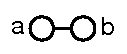
\includegraphics[height=0.4cm]{graph3.pdf}}) with 
vertex labelling with $\pmb{\ell}_{v_1}=a$ and $\pmb{\ell}_{v_2}=b$. We know from 
Corollary~\ref{cor:augmented} that this architecture is upper bounded by 1-WL, starting
from $\pmb{\ell}^{(1)}$. More precisely, we have that $\pmb{\ell}^{(t)}\sqsubseteq\mathbf{F}^{(t-1)}$ for $t\geq 1$.
Consider $\mathbf{F}^{(0)}:=\left(\begin{smallmatrix}1 & 0\\
0 & 1\end{smallmatrix}\right)$ such that $\mathbf{F}^{(0)}$ is good for $\pmb{\ell}$. We also note that $\pmb{\ell}^{(1)}_{v_1}=(a,\{b\})$ and $\pmb{\ell}^{(1)}_{v_2}=(b,\{a\})$. Hence, 
$\mathbf{F}^{(0)}$ is also good for $\pmb{\ell}^{(1)}$. We next show that there does not exists a
weight matrix $\mathbf{W}^{(0)}$ such that $\pmb{\ell}^{(2)}\equiv \mathbf{F}^{(1)}$. Indeed,
$$
\mathbf{F}^{(1)}:=\sigma\Biggl(\frac{1}{2}\biggl(\begin{pmatrix}0 & 1 \\
1 & 0
\end{pmatrix}+
\begin{pmatrix}
	 1 & 0 \\
0 & 1 \end{pmatrix}\biggl)\mathbf{F}^{(0)}\mathbf{W}^{(0)}\Biggr)
=\sigma(\Biggl(\frac{1}{2}\begin{pmatrix}1 & 1 \\
1 & 1
\end{pmatrix}
\mathbf{F}^{(0)}\mathbf{W}^{(0)}\Biggr)=
\sigma\Biggl(\frac{1}{2}\begin{pmatrix}
1& 1\\
1 & 1\\
\end{pmatrix}\mathbf{W}^{(0)}\Biggr).
$$
Hence, independent of the choice of $\mathbf{W}^{(0)}$, both vertices will be assigned the same
feature vector. By contrast, $\pmb{\ell}^{(2)}\sqsubseteq\pmb{\ell}^{(1)}$ and hence
$\pmb{\ell}^{(2)}$ must assign distinct labels to these vertices, since $\pmb{\ell}^{(1)}$ does so. Hence, $\mathbf{F}^{(2)}\not\equiv\pmb{\ell}^{(2)}$.\qed
\end{example}
The example shows that the upper bound for the augmented adjacency architecture as given in Corollary~\ref{cor:augmented} cannot be matched with a lower bound.
In fact the same example can be used to show that the augmented random walk architecture is not as strong as 1-WL, starting from $\pmb{\ell}^{(0)}$. That is the upper bound from Corollary~\ref{cor:augrw1wl} cannot be matched with a lower bound.

In the proof of  Lemma~\ref{lem:findingp} it is also important that $p\neq 0$. THe following simple example shows that the adjacency, random walk and and normalised adjacency architectures are not as strong as 1-WL (recall that for these architectures $p=0$).

\begin{example}\label{example:piszero}
consider the  adjacency architecture on input graph  $(G,\pmb{\ell})$
(\raisebox{-0.4ex}{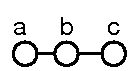
\includegraphics[height=0.5cm]{graph4.pdf}}) with 
vertex labelling with $\pmb{\ell}_{v_1}=a$, $\pmb{\ell}_{v_2}=b$ and $\pmb{\ell}_{v_3}=c$.
Consider $\mathbf{F}^{(0)}:=\left(\begin{smallmatrix}1 & 0 & 0\\
0 & 1 & 0\\
0 & 0 & 1\end{smallmatrix}\right)$ such that $\mathbf{F}^{(0)}$ is good for $\pmb{\ell}$.
Then,
$$
\mathbf{F}^{(1)}:=\sigma\Biggl(\begin{pmatrix}0 & 1 & 0 \\
1 & 0 & 1\\
0 & 1 & 0
\end{pmatrix}\mathbf{F}^{(0)}\mathbf{W}^{(0)}\Biggr)
=\sigma(\mathbf{W}^{(0)}\Biggr)=
\sigma\Biggl(\begin{pmatrix}0 & 1 & 0 \\
1 & 0 & 1\\
0 & 1 & 0
\end{pmatrix}\mathbf{W}^{(0)}\Biggr).
$$
Hence, independent of the choice of $\mathbf{W}^{(0)}$,  vertices $v_1$ and $v_3$ will be assigned the same
feature vector. By contrast, $\pmb{\ell}^{(1)}_{v_1}=(a,\{b\})\neq \pmb{\ell}^{(1)}_{v_2}=(c,\{b\})$.
This example also works for the random walk and and normalised adjacency architectures. \qed
\end{example}

We thus see that having $0<p<1$ is a necessary condition for GNN architectures~(\ref{eq:architecture})
to be as strong as 1-WL.

\subsection{Separating examples}

\openprob{Can we argue, based on results so far how to separate the different GNN models.}
\begin{itemize}
	\item I believe we can use the strongness results do so between the architectures in each group in Table~\ref{tbl:strongGNN}.
	\item It would be great if we can separate all GNNs, even within a group in  Table~\ref{tbl:strongGNN}. Perhaps using $\hat{\pmb{\ell}}$. Also, can one GNN architecture simulate another one? That is, can one find learnable parameters of one model to simulate another one (this is an extension of WL strongness where WL is replaced by the labeling computer by another GNN architecture.) This makes only sense when both GNN architecture are known to be bounded in the same way.
\end{itemize}


\subsection{Bias}
\floris{Perhaps too ambitious...}
\openprob{Can we find examples that show that the bias is needed, i.e., $q\neq 0$ is necessary in general? Note we only need to look at GNN architectures for which $0<p<1$.}
Consider  GNN architectures 
$$\mathbf{F}^{(t+1)}:=\sigma(\mathbf{L}(\mathbf{A}+p\mathbf{I})\mathbf{R}\mathbf{F}^{(t)}\mathbf{W}^{t}),	
$$
with $0<p<1$. We next show that bias is needed.

\begin{example}
	Consider the relaxed augmented random walk architecture
$$\mathbf{F}^{(t+1)}:=\text{sgn}(\tilde{\mathbf{D}}^{-1/2}(\mathbf{A}+p\mathbf{I})\mathbf{F}^{(t)}\mathbf{W}^{t}),
$$
with $0<p<1$. We know that it is upper bounded by 1-WL, starting from $\pmb{\ell}$. We next show that without bias, we cannot get a matching lower bound. Note that this example uses sgn as activation function.

Consider the graph  $(G,\pmb{\ell})$
(\raisebox{-0.4ex}{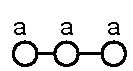
\includegraphics[height=0.5cm]{graph5.pdf}}) with $\pmb{\ell}_{v_1}=\pmb{\ell}_{v_2}=\pmb{\ell}_{v_3}=a$. Let $\mathbf{F}^{(0)}:=\left(\begin{smallmatrix} 1\\1\\1\end{smallmatrix}\right)$.
We have 
$$
\mathbf{F}^{(1)}:=\text{sgn}\Biggl(
\begin{pmatrix}
1/\sqrt{2} & 0 & 0\\
0 & 1/\sqrt{3} & 0\\
0 & 0 & 1/\sqrt{2}
\end{pmatrix}
\begin{pmatrix}
p & 1 & 0\\
1 & p & 1\\
0 & 1 & p
\end{pmatrix}
\begin{pmatrix}
	1\\
	1\\
	1
	\end{pmatrix}\mathbf{W}^{(0)}\Biggr)
=\text{sgn}\Biggl(
\begin{pmatrix}
\frac{1}{\sqrt{2}}(1+p)\\
\frac{1}{\sqrt{3}}(2+p)\\
\frac{1}{\sqrt{2}}(1+p)\end{pmatrix}
\mathbf{W}^{(0)}
\Biggr)
$$
We remark that $\mathbf{W}^{(0)}$ is a $1\times f$-matrix. Clearly, all entries in
$\mathbf{F}^{(1)}$ will have the same sign. By contrast, $\pmb{\ell}^{(1)}_{v_1}=(a,\{a\})\neq
(a,\{a,a\})=\pmb{\ell}^{(1)}_{v_2}$. So, $\pmb{\ell}^{(1)}\not\equiv\mathbf{F}^{(1)}$ for any choice of $\mathbf{W}^{(0)}$.\qed
\end{example}

% \begin{corollary}
% Suppose that $\pmb{\ell}\not\equiv\hat{\pmb{\ell}}$ but $\pmb{\ell}^{(1)}\sqsubseteq \hat{\pmb{\ell}}$. Then, the architecture is bounded by 1-WL, starting from $\pmb{\ell}^{(1)}$.
% \end{corollary}
% \begin{proof}
% Let $t=0$. We have that $\pmb{\ell}^{(1)}\sqsubseteq \pmb{\ell}\sqsubset \mathbf{F}^{(0)}$. For $t=1$, assume that $\pmb{\ell}^{(2)}_v=\pmb{\ell}^{(2)}_w$. We show that
% $\mathbf{F}_{v\bullet}^{(1)}=\mathbf{F}_{w\bullet}^{(1)}$.
% Indeed, we have that $\pmb{\ell}^{(1)}_v=\pmb{\ell}^{(1)}_w$ and
%  for every $u\in N_G(v)$ and corresponding $u'\in N_G(w)$,
%  $\pmb{\ell}^{(1)}_u=\pmb{\ell}^{(1)}_{u'}$. Then,
%  $\pmb{\ell}^{(1)}\sqsubseteq \hat{\pmb{\ell}}$ implies that
%   $\mathbf{L}_{vv}=\mathbf{L}_{ww}$, $\mathbf{R}_{vv}=\mathbf{R}_{ww}$ and
% $\mathbf{B}_{v\bullet}=\mathbf{B}_{w\bullet}$.
% Furthermore, for every $u\in N_G(v)$ and corresponding $u'\in N_G(w)$, $\mathbf{R}_{uu}=\mathbf{R}_{u'u'}$. By induction, also $\pmb{\ell}^{(1)}\subseteq \mathbf{F}^{(0)}$. This suffices to conclude that $\mathbf{F}^{(1)}_{v\bullet}=\mathbf{F}^{(1)}_{w\bullet}$. For $t>2$, assume that $\pmb{\ell}^{(t)}_v=\pmb{\ell}^{(t)}_w$. Then,
%  $\pmb{\ell}^{(t-1)}_v=\pmb{\ell}^{(t-1)}_w$ and for every $u\in N_G(v)$ and corresponding $u'\in N_G(w)$,  $\pmb{\ell}^{(t-1)}_u=\pmb{\ell}^{(t-1)}_{u'}$. In particular,
%  since $\pmb{\ell}^{(t-1)}\sqsubseteq \pmb{\ell}^{(1)}$,
%  $\pmb{\ell}^{(1)}_v=\pmb{\ell}^{(1)}_w$ and for every $u\in N_G(v)$ and corresponding $u'\in N_G(w)$,  $\pmb{\ell}^{(1)}_u=\pmb{\ell}^{(1)}_{u'}$. Using that $\pmb{\ell}^{(1)}\sqsubseteq \hat{\pmb{\ell}}$ holds, this implies that
%  $\mathbf{L}_{vv}=\mathbf{L}_{ww}$, $\mathbf{R}_{vv}=\mathbf{R}_{ww}$ and
% $\mathbf{B}_{v\bullet}=\mathbf{B}_{w\bullet}$. Furthermore, for every $u\in N_G(v)$ and corresponding $u'\in N_G(w)$, $\mathbf{R}_{uu}=\mathbf{R}_{u'u'}$. By induction, also $\pmb{\ell}^{(t-1)}\subseteq \mathbf{F}^{(t-2)}$. This suffices to conclude that $\mathbf{F}^{(t-1)}_{v\bullet}=\mathbf{F}^{(t-1)}_{w\bullet}$.
% \end{proof}
% This corollary applies, for example, for the normalized adjacency and augmented adjacency architecture.

%
% \todo{From an upper bound perspective, $\mathbf{L}$ has no apparent impact when it is degree related. By contrast, $\mathbf{R}$ speeds up
% 1-WL with one step. The role of $p$ and $q$ and $\mathbf{B}$ also do seem to have an impact for upper bounds. Can we say something more here?}
%!TEX root = quiver.tex
